\documentclass[border=0pt]{standalone}
\usepackage{iftex}
\ifPDFTeX
  \usepackage[T1]{fontenc}
  \usepackage{DejaVuSans}
  \renewcommand*\familydefault{\sfdefault}
  \usepackage[italic]{mathastext}
\else
  \usepackage{unicode-math}
  \setmainfont{DejaVuSans.ttf}[BoldFont=DejaVuSans-Bold.ttf,ItalicFont=DejaVuSans-Oblique.ttf,
    BoldItalicFont=DejaVuSans-BoldOblique.ttf]
  \setmathfont{texgyredejavu-math.otf}
\fi
\ifPDFTeX  % one glyph of matplotlib mathtext, by Unicode code point (hex)
  \def\mplchar#1{\ifnum"#1="2212 \ensuremath{-}\else\ifnum"#1="D7 \texttimes\else\char"#1\relax\fi\fi}
\else
  \def\mplchar#1{\char"#1\relax}
\fi
\frenchspacing  % matplotlib puts a normal space after punctuation
\usepackage{pgfplots}
\pgfplotsset{compat=1.18}
% matplotlib marker shapes; \pgfplotmarksize = half the matplotlib marker size
\pgfdeclareplotmark{mpl-o}{\pgfpathcircle{\pgfpointorigin}{\pgfplotmarksize}\pgfusepathqfillstroke}
\pgfdeclareplotmark{mpl-o-open}{\pgfpathcircle{\pgfpointorigin}{\pgfplotmarksize}\pgfusepathqstroke}
\pgfdeclareplotmark{mpl-s}{\pgfpathrectangle{\pgfpoint{-\pgfplotmarksize}{-\pgfplotmarksize}}{\pgfpoint{2\pgfplotmarksize}{2\pgfplotmarksize}}\pgfusepathqfillstroke}
\pgfdeclareplotmark{mpl-s-open}{\pgfpathrectangle{\pgfpoint{-\pgfplotmarksize}{-\pgfplotmarksize}}{\pgfpoint{2\pgfplotmarksize}{2\pgfplotmarksize}}\pgfusepathqstroke}
\def\mpltriangle#1{\pgfpathmoveto{\pgfpoint{0pt}{#1\pgfplotmarksize}}\pgfpathlineto{\pgfpoint{-\pgfplotmarksize}{-#1\pgfplotmarksize}}\pgfpathlineto{\pgfpoint{\pgfplotmarksize}{-#1\pgfplotmarksize}}\pgfpathclose}
\pgfdeclareplotmark{mpl-^}{\mpltriangle{}\pgfusepathqfillstroke}
\pgfdeclareplotmark{mpl-^-open}{\mpltriangle{}\pgfusepathqstroke}
\pgfdeclareplotmark{mpl-v}{\mpltriangle{-}\pgfusepathqfillstroke}
\pgfdeclareplotmark{mpl-v-open}{\mpltriangle{-}\pgfusepathqstroke}
\def\mpldiamond{\pgfpathmoveto{\pgfpoint{0pt}{1.41421\pgfplotmarksize}}\pgfpathlineto{\pgfpoint{-1.41421\pgfplotmarksize}{0pt}}\pgfpathlineto{\pgfpoint{0pt}{-1.41421\pgfplotmarksize}}\pgfpathlineto{\pgfpoint{1.41421\pgfplotmarksize}{0pt}}\pgfpathclose}
\pgfdeclareplotmark{mpl-D}{\mpldiamond\pgfusepathqfillstroke}
\pgfdeclareplotmark{mpl-D-open}{\mpldiamond\pgfusepathqstroke}
\pgfdeclareplotmark{mpl-x}{\pgfpathmoveto{\pgfpoint{-\pgfplotmarksize}{-\pgfplotmarksize}}\pgfpathlineto{\pgfpoint{\pgfplotmarksize}{\pgfplotmarksize}}\pgfpathmoveto{\pgfpoint{-\pgfplotmarksize}{\pgfplotmarksize}}\pgfpathlineto{\pgfpoint{\pgfplotmarksize}{-\pgfplotmarksize}}\pgfsetbuttcap\pgfusepathqstroke}
\pgfdeclareplotmark{mpl-+}{\pgfpathmoveto{\pgfpoint{-\pgfplotmarksize}{0pt}}\pgfpathlineto{\pgfpoint{\pgfplotmarksize}{0pt}}\pgfpathmoveto{\pgfpoint{0pt}{-\pgfplotmarksize}}\pgfpathlineto{\pgfpoint{0pt}{\pgfplotmarksize}}\pgfsetbuttcap\pgfusepathqstroke}
\def\mplplus{\pgfpathmoveto{\pgfpoint{-0.33333\pgfplotmarksize}{-\pgfplotmarksize}}\pgfpathlineto{\pgfpoint{0.33333\pgfplotmarksize}{-\pgfplotmarksize}}\pgfpathlineto{\pgfpoint{0.33333\pgfplotmarksize}{-0.33333\pgfplotmarksize}}\pgfpathlineto{\pgfpoint{\pgfplotmarksize}{-0.33333\pgfplotmarksize}}\pgfpathlineto{\pgfpoint{\pgfplotmarksize}{0.33333\pgfplotmarksize}}\pgfpathlineto{\pgfpoint{0.33333\pgfplotmarksize}{0.33333\pgfplotmarksize}}\pgfpathlineto{\pgfpoint{0.33333\pgfplotmarksize}{\pgfplotmarksize}}\pgfpathlineto{\pgfpoint{-0.33333\pgfplotmarksize}{\pgfplotmarksize}}\pgfpathlineto{\pgfpoint{-0.33333\pgfplotmarksize}{0.33333\pgfplotmarksize}}\pgfpathlineto{\pgfpoint{-\pgfplotmarksize}{0.33333\pgfplotmarksize}}\pgfpathlineto{\pgfpoint{-\pgfplotmarksize}{-0.33333\pgfplotmarksize}}\pgfpathlineto{\pgfpoint{-0.33333\pgfplotmarksize}{-0.33333\pgfplotmarksize}}\pgfpathclose}
\pgfdeclareplotmark{mpl-P}{\mplplus\pgfusepathqfillstroke}
\pgfdeclareplotmark{mpl-P-open}{\mplplus\pgfusepathqstroke}
\def\mplstar{\pgfpathmoveto{\pgfpointpolar{90}{\pgfplotmarksize}}%
  \foreach \i in {1,...,4} {\pgfpathlineto{\pgfpointpolar{90+72*\i-36}{0.381966\pgfplotmarksize}}\pgfpathlineto{\pgfpointpolar{90+72*\i}{\pgfplotmarksize}}}%
  \pgfpathlineto{\pgfpointpolar{54}{0.381966\pgfplotmarksize}}\pgfpathclose}
\pgfdeclareplotmark{mpl-*}{\mplstar\pgfusepathqfillstroke}
\pgfdeclareplotmark{mpl-*-open}{\mplstar\pgfusepathqstroke}
\def\mpltriside#1{\pgfpathmoveto{\pgfpoint{#1\pgfplotmarksize}{0pt}}\pgfpathlineto{\pgfpoint{-#1\pgfplotmarksize}{\pgfplotmarksize}}\pgfpathlineto{\pgfpoint{-#1\pgfplotmarksize}{-\pgfplotmarksize}}\pgfpathclose}
\pgfdeclareplotmark{mpl-<}{\mpltriside{-}\pgfusepathqfillstroke}
\pgfdeclareplotmark{mpl-<-open}{\mpltriside{-}\pgfusepathqstroke}
\pgfdeclareplotmark{mpl->}{\mpltriside{}\pgfusepathqfillstroke}
\pgfdeclareplotmark{mpl->-open}{\mpltriside{}\pgfusepathqstroke}
\def\mplpolygon#1{\pgfpathmoveto{\pgfpointpolar{90}{\pgfplotmarksize}}\foreach \i in {1,...,#1} {\pgfpathlineto{\pgfpointpolar{90+360/#1*\i}{\pgfplotmarksize}}}\pgfpathclose}
\pgfdeclareplotmark{mpl-p}{\mplpolygon{5}\pgfusepathqfillstroke}
\pgfdeclareplotmark{mpl-p-open}{\mplpolygon{5}\pgfusepathqstroke}
\pgfdeclareplotmark{mpl-h}{\mplpolygon{6}\pgfusepathqfillstroke}
\pgfdeclareplotmark{mpl-h-open}{\mplpolygon{6}\pgfusepathqstroke}
\definecolor{mplc0}{HTML}{B0B0B0}
\definecolor{mplc1}{HTML}{000000}
\definecolor{mplc2}{HTML}{1F77B4}
\definecolor{mplc3}{HTML}{D62728}
\definecolor{mplc4}{HTML}{DAA520}
\definecolor{mplc5}{HTML}{9467BD}
\definecolor{mplc6}{HTML}{17BECF}
\definecolor{mplc7}{HTML}{2CA02C}
\begin{document}
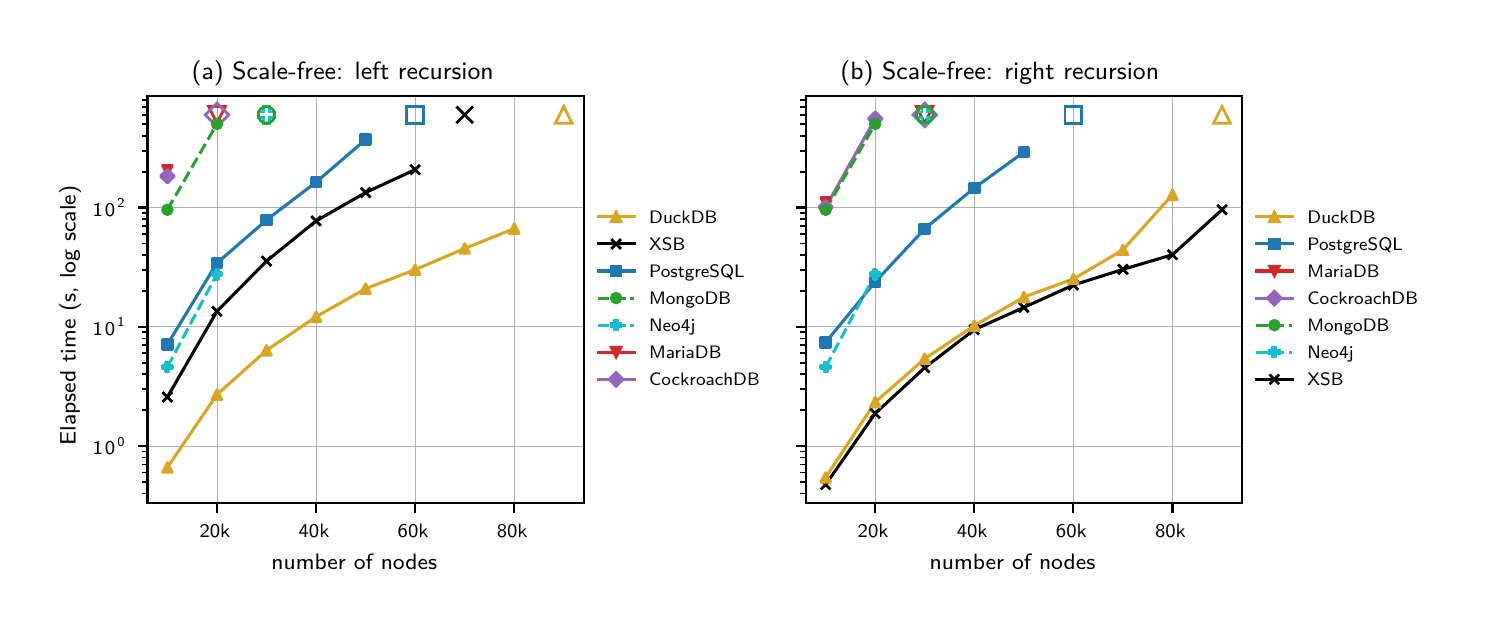
\begin{tikzpicture}
\useasboundingbox (0in,0in) rectangle (7.2in,2.9in);
\begin{axis}[at={(0.5995in,0.5228in)}, anchor=south west, scale only axis, width=2.1802in, height=2.0338in, xmin=6000, xmax=94000, ymin=0.3316568615, ymax=857.5678697, enlargelimits=false, clip=true, axis on top=false, axis line style={line width=0.8bp, black}, tick align=outside, tick pos=left, major tick length=3.5bp, minor tick length=2bp, major tick style={line width=0.8bp, black}, minor tick style={line width=0.6bp, black}, xticklabels={}, yticklabels={}, scaled x ticks=false, scaled y ticks=false, xlabel={}, ylabel={}, title={}, xtick={20000,40000,60000,80000}, minor xtick={}, ymode=log, log basis y=10, ytick={1,10,100}, minor ytick={0.4,0.5,0.6,0.7,0.8,0.9,2,3,4,5,6,7,8,9,20,30,40,50,60,70,80,90,200,300,400,500,600,700,800}, xmajorgrids, ymajorgrids, major grid style={line width=0.3bp, draw=mplc0}]
\addplot[color=mplc1, line width=1.1bp, line join=round, solid, line cap=rect, mark=mpl-x, mark size=1.75bp, mark options={solid, line width=1bp, draw=mplc1}] coordinates {(10000,2.574047327) (20000,13.48110833) (30000,35.53593583) (40000,77.27983842) (50000,133.7014546) (60000,208.1350324)};
\addplot[only marks, mark=mpl-x, mark size=3bp, mark options={solid, line width=1bp, draw=mplc1}] coordinates {(70000,600)};
\addplot[color=mplc2, line width=1.1bp, line join=round, solid, line cap=rect, mark=mpl-s, mark size=1.75bp, mark options={solid, line width=1bp, draw=mplc2, fill=mplc2}] coordinates {(10000,7.109274433) (20000,34.27205188) (30000,78.56963498) (40000,163.4126305) (50000,372.0274507)};
\addplot[only marks, mark=mpl-s-open, mark size=3bp, mark options={solid, line width=1bp, draw=mplc2}] coordinates {(60000,600)};
\addplot[color=mplc3, line width=1.1bp, line join=round, solid, line cap=rect, mark=mpl-v, mark size=1.75bp, mark options={solid, line width=1bp, draw=mplc3, fill=mplc3}] coordinates {(10000,205.6145777)};
\addplot[only marks, mark=mpl-v-open, mark size=3bp, mark options={solid, line width=1bp, draw=mplc3}] coordinates {(20000,600)};
\addplot[color=mplc4, line width=1.1bp, line join=round, solid, line cap=rect, mark=mpl-^, mark size=1.75bp, mark options={solid, line width=1bp, draw=mplc4, fill=mplc4}] coordinates {(10000,0.6606844416) (20000,2.697761667) (30000,6.346119558) (40000,12.13651263) (50000,20.86290837) (60000,30.14692048) (70000,45.41494353) (80000,66.65669588)};
\addplot[only marks, mark=mpl-^-open, mark size=3bp, mark options={solid, line width=1bp, draw=mplc4}] coordinates {(90000,600)};
\addplot[color=mplc5, line width=1.1bp, line join=round, solid, line cap=rect, mark=mpl-D, mark size=1.75bp, mark options={solid, line width=1bp, draw=mplc5, fill=mplc5}] coordinates {(10000,183.7256635)};
\addplot[only marks, mark=mpl-D-open, mark size=3bp, mark options={solid, line width=1bp, draw=mplc5}] coordinates {(20000,600)};
\addplot[color=mplc6, line width=1.1bp, line join=round, dash pattern=on 4.07bp off 1.76bp, line cap=butt, mark=mpl-P, mark size=1.75bp, mark options={solid, line width=1bp, draw=mplc6, fill=mplc6}] coordinates {(10000,4.595514983) (20000,27.58427781)};
\addplot[only marks, mark=mpl-P-open, mark size=3bp, mark options={solid, line width=1bp, draw=mplc6}] coordinates {(30000,600)};
\addplot[color=mplc7, line width=1.1bp, line join=round, dash pattern=on 4.07bp off 1.76bp, line cap=butt, mark=mpl-o, mark size=1.75bp, mark options={solid, line width=1bp, draw=mplc7, fill=mplc7}] coordinates {(10000,95.88224765) (20000,502.8930846)};
\addplot[only marks, mark=mpl-o-open, mark size=3bp, mark options={solid, line width=1bp, draw=mplc7}] coordinates {(30000,600)};
\end{axis}
\begin{axis}[at={(3.8907in,0.5228in)}, anchor=south west, scale only axis, width=2.1802in, height=2.0338in, xmin=6000, xmax=94000, ymin=0.3316568615, ymax=857.5678697, enlargelimits=false, clip=true, axis on top=false, axis line style={line width=0.8bp, black}, tick align=outside, tick pos=left, major tick length=3.5bp, minor tick length=2bp, major tick style={line width=0.8bp, black}, minor tick style={line width=0.6bp, black}, xticklabels={}, yticklabels={}, scaled x ticks=false, scaled y ticks=false, xlabel={}, ylabel={}, title={}, xtick={20000,40000,60000,80000}, minor xtick={}, ymode=log, log basis y=10, ytick={1,10,100}, minor ytick={0.4,0.5,0.6,0.7,0.8,0.9,2,3,4,5,6,7,8,9,20,30,40,50,60,70,80,90,200,300,400,500,600,700,800}, xmajorgrids, ymajorgrids, major grid style={line width=0.3bp, draw=mplc0}]
\addplot[color=mplc1, line width=1.1bp, line join=round, solid, line cap=rect, mark=mpl-x, mark size=1.75bp, mark options={solid, line width=1bp, draw=mplc1}] coordinates {(10000,0.474030447) (20000,1.875688982) (30000,4.537005949) (40000,9.45919137) (50000,14.53438401) (60000,22.3968596) (70000,30.32453656) (80000,40.21459641) (90000,95.92929535)};
\addplot[color=mplc2, line width=1.1bp, line join=round, solid, line cap=rect, mark=mpl-s, mark size=1.75bp, mark options={solid, line width=1bp, draw=mplc2, fill=mplc2}] coordinates {(10000,7.39167265) (20000,23.80505083) (30000,66.44698574) (40000,145.9814249) (50000,291.6705084)};
\addplot[only marks, mark=mpl-s-open, mark size=3bp, mark options={solid, line width=1bp, draw=mplc2}] coordinates {(60000,600)};
\addplot[color=mplc3, line width=1.1bp, line join=round, solid, line cap=rect, mark=mpl-v, mark size=1.75bp, mark options={solid, line width=1bp, draw=mplc3, fill=mplc3}] coordinates {(10000,110.4153453)};
\addplot[only marks, mark=mpl-v-open, mark size=3bp, mark options={solid, line width=1bp, draw=mplc3}] coordinates {(30000,600)};
\addplot[color=mplc4, line width=1.1bp, line join=round, solid, line cap=rect, mark=mpl-^, mark size=1.75bp, mark options={solid, line width=1bp, draw=mplc4, fill=mplc4}] coordinates {(10000,0.544465525) (20000,2.329703933) (30000,5.395763683) (40000,10.22430052) (50000,17.74615161) (60000,25.20702907) (70000,44.14625139) (80000,128.0719837)};
\addplot[only marks, mark=mpl-^-open, mark size=3bp, mark options={solid, line width=1bp, draw=mplc4}] coordinates {(90000,600)};
\addplot[color=mplc5, line width=1.1bp, line join=round, solid, line cap=rect, mark=mpl-D, mark size=1.75bp, mark options={solid, line width=1bp, draw=mplc5, fill=mplc5}] coordinates {(10000,100.8391892) (20000,556.577931)};
\addplot[only marks, mark=mpl-D-open, mark size=3bp, mark options={solid, line width=1bp, draw=mplc5}] coordinates {(30000,600)};
\addplot[color=mplc6, line width=1.1bp, line join=round, dash pattern=on 4.07bp off 1.76bp, line cap=butt, mark=mpl-P, mark size=1.75bp, mark options={solid, line width=1bp, draw=mplc6, fill=mplc6}] coordinates {(10000,4.595514983) (20000,27.58427781)};
\addplot[only marks, mark=mpl-P-open, mark size=3bp, mark options={solid, line width=1bp, draw=mplc6}] coordinates {(30000,600)};
\addplot[color=mplc7, line width=1.1bp, line join=round, dash pattern=on 4.07bp off 1.76bp, line cap=butt, mark=mpl-o, mark size=1.75bp, mark options={solid, line width=1bp, draw=mplc7, fill=mplc7}] coordinates {(10000,95.88224765) (20000,502.8930846)};
\addplot[only marks, mark=mpl-o-open, mark size=3bp, mark options={solid, line width=1bp, draw=mplc7}] coordinates {(30000,600)};
\end{axis}
\draw[color=mplc4, line width=1.1bp, line join=round, solid, line cap=rect] (2.8519in,1.9541in) -- (3.0325in,1.9541in);
\begin{scope}[solid, line width=1bp, draw=mplc4, fill=mplc4]\pgftransformshift{\pgfpoint{2.9422in}{1.9541in}}\pgfsetplotmarksize{1.75bp}\pgfuseplotmark{mpl-^}\end{scope}
\draw[color=mplc1, line width=1.1bp, line join=round, solid, line cap=rect] (2.8519in,1.8187in) -- (3.0325in,1.8187in);
\begin{scope}[solid, line width=1bp, draw=mplc1]\pgftransformshift{\pgfpoint{2.9422in}{1.8187in}}\pgfsetplotmarksize{1.75bp}\pgfuseplotmark{mpl-x}\end{scope}
\draw[color=mplc2, line width=1.1bp, line join=round, solid, line cap=rect] (2.8519in,1.6833in) -- (3.0325in,1.6833in);
\begin{scope}[solid, line width=1bp, draw=mplc2, fill=mplc2]\pgftransformshift{\pgfpoint{2.9422in}{1.6833in}}\pgfsetplotmarksize{1.75bp}\pgfuseplotmark{mpl-s}\end{scope}
\draw[color=mplc7, line width=1.1bp, line join=round, dash pattern=on 4.07bp off 1.76bp, line cap=butt] (2.8519in,1.5479in) -- (3.0325in,1.5479in);
\begin{scope}[solid, line width=1bp, draw=mplc7, fill=mplc7]\pgftransformshift{\pgfpoint{2.9422in}{1.5479in}}\pgfsetplotmarksize{1.75bp}\pgfuseplotmark{mpl-o}\end{scope}
\draw[color=mplc6, line width=1.1bp, line join=round, dash pattern=on 4.07bp off 1.76bp, line cap=butt] (2.8519in,1.4125in) -- (3.0325in,1.4125in);
\begin{scope}[solid, line width=1bp, draw=mplc6, fill=mplc6]\pgftransformshift{\pgfpoint{2.9422in}{1.4125in}}\pgfsetplotmarksize{1.75bp}\pgfuseplotmark{mpl-P}\end{scope}
\draw[color=mplc3, line width=1.1bp, line join=round, solid, line cap=rect] (2.8519in,1.2771in) -- (3.0325in,1.2771in);
\begin{scope}[solid, line width=1bp, draw=mplc3, fill=mplc3]\pgftransformshift{\pgfpoint{2.9422in}{1.2771in}}\pgfsetplotmarksize{1.75bp}\pgfuseplotmark{mpl-v}\end{scope}
\draw[color=mplc5, line width=1.1bp, line join=round, solid, line cap=rect] (2.8519in,1.1416in) -- (3.0325in,1.1416in);
\begin{scope}[solid, line width=1bp, draw=mplc5, fill=mplc5]\pgftransformshift{\pgfpoint{2.9422in}{1.1416in}}\pgfsetplotmarksize{1.75bp}\pgfuseplotmark{mpl-D}\end{scope}
\draw[color=mplc4, line width=1.1bp, line join=round, solid, line cap=rect] (6.1431in,1.9541in) -- (6.3237in,1.9541in);
\begin{scope}[solid, line width=1bp, draw=mplc4, fill=mplc4]\pgftransformshift{\pgfpoint{6.2334in}{1.9541in}}\pgfsetplotmarksize{1.75bp}\pgfuseplotmark{mpl-^}\end{scope}
\draw[color=mplc2, line width=1.1bp, line join=round, solid, line cap=rect] (6.1431in,1.8187in) -- (6.3237in,1.8187in);
\begin{scope}[solid, line width=1bp, draw=mplc2, fill=mplc2]\pgftransformshift{\pgfpoint{6.2334in}{1.8187in}}\pgfsetplotmarksize{1.75bp}\pgfuseplotmark{mpl-s}\end{scope}
\draw[color=mplc3, line width=1.1bp, line join=round, solid, line cap=rect] (6.1431in,1.6833in) -- (6.3237in,1.6833in);
\begin{scope}[solid, line width=1bp, draw=mplc3, fill=mplc3]\pgftransformshift{\pgfpoint{6.2334in}{1.6833in}}\pgfsetplotmarksize{1.75bp}\pgfuseplotmark{mpl-v}\end{scope}
\draw[color=mplc5, line width=1.1bp, line join=round, solid, line cap=rect] (6.1431in,1.5479in) -- (6.3237in,1.5479in);
\begin{scope}[solid, line width=1bp, draw=mplc5, fill=mplc5]\pgftransformshift{\pgfpoint{6.2334in}{1.5479in}}\pgfsetplotmarksize{1.75bp}\pgfuseplotmark{mpl-D}\end{scope}
\draw[color=mplc7, line width=1.1bp, line join=round, dash pattern=on 4.07bp off 1.76bp, line cap=butt] (6.1431in,1.4125in) -- (6.3237in,1.4125in);
\begin{scope}[solid, line width=1bp, draw=mplc7, fill=mplc7]\pgftransformshift{\pgfpoint{6.2334in}{1.4125in}}\pgfsetplotmarksize{1.75bp}\pgfuseplotmark{mpl-o}\end{scope}
\draw[color=mplc6, line width=1.1bp, line join=round, dash pattern=on 4.07bp off 1.76bp, line cap=butt] (6.1431in,1.2771in) -- (6.3237in,1.2771in);
\begin{scope}[solid, line width=1bp, draw=mplc6, fill=mplc6]\pgftransformshift{\pgfpoint{6.2334in}{1.2771in}}\pgfsetplotmarksize{1.75bp}\pgfuseplotmark{mpl-P}\end{scope}
\draw[color=mplc1, line width=1.1bp, line join=round, solid, line cap=rect] (6.1431in,1.1416in) -- (6.3237in,1.1416in);
\begin{scope}[solid, line width=1bp, draw=mplc1]\pgftransformshift{\pgfpoint{6.2334in}{1.1416in}}\pgfsetplotmarksize{1.75bp}\pgfuseplotmark{mpl-x}\end{scope}
\node[anchor=base west, inner sep=0pt, text=mplc1, font=\fontsize{7bp}{8.4bp}\selectfont] at (0.8564in,0.3517in) {20k};
\node[anchor=base west, inner sep=0pt, text=mplc1, font=\fontsize{7bp}{8.4bp}\selectfont] at (1.3519in,0.3517in) {40k};
\node[anchor=base west, inner sep=0pt, text=mplc1, font=\fontsize{7bp}{8.4bp}\selectfont] at (1.8474in,0.3517in) {60k};
\node[anchor=base west, inner sep=0pt, text=mplc1, font=\fontsize{7bp}{8.4bp}\selectfont] at (2.3429in,0.3517in) {80k};
\node[anchor=base west, inner sep=0pt, text=mplc1, font=\fontsize{8bp}{9.6bp}\selectfont] at (1.2161in,0.1884in) {number of nodes};
\node[anchor=base west, inner sep=0pt, text=mplc1, font=\fontsize{7bp}{8.4bp}\selectfont] at (0.3217in,0.7664in) {\mplchar{31}};
\node[anchor=base west, inner sep=0pt, text=mplc1, font=\fontsize{7bp}{8.4bp}\selectfont] at (0.3835in,0.7664in) {\mplchar{30}};
\node[anchor=base west, inner sep=0pt, text=mplc1, font=\fontsize{4.9bp}{5.88bp}\selectfont] at (0.4463in,0.8065in) {\mplchar{30}};
\node[anchor=base west, inner sep=0pt, text=mplc1, font=\fontsize{7bp}{8.4bp}\selectfont] at (0.3217in,1.3633in) {\mplchar{31}};
\node[anchor=base west, inner sep=0pt, text=mplc1, font=\fontsize{7bp}{8.4bp}\selectfont] at (0.3835in,1.3633in) {\mplchar{30}};
\node[anchor=base west, inner sep=0pt, text=mplc1, font=\fontsize{4.9bp}{5.88bp}\selectfont] at (0.4463in,1.4034in) {\mplchar{31}};
\node[anchor=base west, inner sep=0pt, text=mplc1, font=\fontsize{7bp}{8.4bp}\selectfont] at (0.3217in,1.9583in) {\mplchar{31}};
\node[anchor=base west, inner sep=0pt, text=mplc1, font=\fontsize{7bp}{8.4bp}\selectfont] at (0.3835in,1.9583in) {\mplchar{30}};
\node[anchor=base west, inner sep=0pt, text=mplc1, font=\fontsize{4.9bp}{5.88bp}\selectfont] at (0.4463in,1.9985in) {\mplchar{32}};
\node[anchor=base west, inner sep=0pt, rotate=90, text=mplc1, font=\fontsize{8bp}{9.6bp}\selectfont] at (0.2394in,0.8072in) {Elapsed time (s, log scale)};
\node[anchor=base west, inner sep=0pt, text=mplc1, font=\fontsize{9bp}{10.8bp}\selectfont] at (0.8165in,2.64in) {(a) Scale-free: left recursion};
\node[anchor=base west, inner sep=0pt, text=mplc1, font=\fontsize{6.5bp}{7.8bp}\selectfont] at (3.1047in,1.9225in) {DuckDB};
\node[anchor=base west, inner sep=0pt, text=mplc1, font=\fontsize{6.5bp}{7.8bp}\selectfont] at (3.1047in,1.7871in) {XSB};
\node[anchor=base west, inner sep=0pt, text=mplc1, font=\fontsize{6.5bp}{7.8bp}\selectfont] at (3.1047in,1.6517in) {PostgreSQL};
\node[anchor=base west, inner sep=0pt, text=mplc1, font=\fontsize{6.5bp}{7.8bp}\selectfont] at (3.1047in,1.5163in) {MongoDB};
\node[anchor=base west, inner sep=0pt, text=mplc1, font=\fontsize{6.5bp}{7.8bp}\selectfont] at (3.1047in,1.3809in) {Neo4j};
\node[anchor=base west, inner sep=0pt, text=mplc1, font=\fontsize{6.5bp}{7.8bp}\selectfont] at (3.1047in,1.2455in) {MariaDB};
\node[anchor=base west, inner sep=0pt, text=mplc1, font=\fontsize{6.5bp}{7.8bp}\selectfont] at (3.1047in,1.11in) {CockroachDB};
\node[anchor=base west, inner sep=0pt, text=mplc1, font=\fontsize{7bp}{8.4bp}\selectfont] at (4.1476in,0.3517in) {20k};
\node[anchor=base west, inner sep=0pt, text=mplc1, font=\fontsize{7bp}{8.4bp}\selectfont] at (4.6431in,0.3517in) {40k};
\node[anchor=base west, inner sep=0pt, text=mplc1, font=\fontsize{7bp}{8.4bp}\selectfont] at (5.1386in,0.3517in) {60k};
\node[anchor=base west, inner sep=0pt, text=mplc1, font=\fontsize{7bp}{8.4bp}\selectfont] at (5.6341in,0.3517in) {80k};
\node[anchor=base west, inner sep=0pt, text=mplc1, font=\fontsize{8bp}{9.6bp}\selectfont] at (4.5073in,0.1884in) {number of nodes};
\node[anchor=base west, inner sep=0pt, text=mplc1, font=\fontsize{9bp}{10.8bp}\selectfont] at (4.0607in,2.64in) {(b) Scale-free: right recursion};
\node[anchor=base west, inner sep=0pt, text=mplc1, font=\fontsize{6.5bp}{7.8bp}\selectfont] at (6.3959in,1.9225in) {DuckDB};
\node[anchor=base west, inner sep=0pt, text=mplc1, font=\fontsize{6.5bp}{7.8bp}\selectfont] at (6.3959in,1.7871in) {PostgreSQL};
\node[anchor=base west, inner sep=0pt, text=mplc1, font=\fontsize{6.5bp}{7.8bp}\selectfont] at (6.3959in,1.6517in) {MariaDB};
\node[anchor=base west, inner sep=0pt, text=mplc1, font=\fontsize{6.5bp}{7.8bp}\selectfont] at (6.3959in,1.5163in) {CockroachDB};
\node[anchor=base west, inner sep=0pt, text=mplc1, font=\fontsize{6.5bp}{7.8bp}\selectfont] at (6.3959in,1.3809in) {MongoDB};
\node[anchor=base west, inner sep=0pt, text=mplc1, font=\fontsize{6.5bp}{7.8bp}\selectfont] at (6.3959in,1.2455in) {Neo4j};
\node[anchor=base west, inner sep=0pt, text=mplc1, font=\fontsize{6.5bp}{7.8bp}\selectfont] at (6.3959in,1.11in) {XSB};
\end{tikzpicture}
\end{document}
